\documentclass[a4paper,10pt]{article}
\usepackage[utf8]{inputenc}
\usepackage{fullpage}
 \usepackage{latexsym,mathrsfs}
\usepackage{amssymb,amsfonts,amsmath,bm}
\usepackage{natbib}
\usepackage{algorithm}
\usepackage{algpseudocode}
\usepackage{algorithmicx}
\usepackage{color}
\usepackage{graphics}
\usepackage{graphicx}
\usepackage{bbm}
%opening
\title{A note on the use of warping to impose Dirichlet conditions on Gaussian Processes}
\author{Victor Picheny}

\def\ds{\displaystyle}
\def\R{\mathbb{R}}
\newcommand{\x}{\mathbf{x}}
\newcommand{\X}{\mathbf{X}}
\newcommand{\y}{\mathbf{y}}
\newcommand{\cc}{\mathbf{c}}
\newcommand{\f}{\mathbf{f}}
\newcommand{\Y}{\mathbf{Y}}
\newcommand{\F}{\mathbf{F}}
\newcommand{\z}{\mathbf{z}}
\newcommand{\s}{\mathbf{x}}
\newcommand{\Sset}{\mathbb{X}}
\newcommand{\Rset}{\mathbb{R}}
\newcommand{\Xset}{\mathbb{X}}
\newcommand{\Prob}{\mathbb{P}}
\newcommand{\yr}{\mathcal{Y}}
\newcommand{\fr}{\mathcal{F}}
\newcommand{\Fr}{\boldsymbol{\mathcal{F}}}
\newcommand{\Yr}{\boldsymbol{\mathcal{Y}}}
\newcommand{\xr}{\mathcal{X}}
\newcommand{\sr}{\mathbb{X}}
\newcommand{\new}{_{\text{new}}}
\newcommand{\cand}{_{\text{cand}}}
\newcommand{\esp}{\mathbb{E}}
\newcommand{\xlarge}{\mathbb{X}_\text{large}}
\def\cov{\operatorname{cov}}
\def\diag{\operatorname{diag}}
\def\card{\operatorname{Card}}

\begin{document}
\maketitle

\section{Motivating problem}
We consider an optimization problem of the type $\min y(\x)$ such that $\x \in \Xset \subset \Rset^d$.
We assume that $\Xset$ is a hyperrectangle.

For some values of a subset of parameters, it is known that $y$ is insensitive to another subset of parameters. 
Take for instance a function that depends on two discs, parameterized by $x_1=r_1 \in [0, r_{\max}]$ (radius of the first disc) and $x_2=\rho_{12} \in [0,1]$ 
(ratio between $r_1$ and the radius of the second disc, $r_2$). Setting $x_1=0$, we have $r_2=0$ for any value of $\rho_{12}$, so $y(0, x_2)$ is constant.

We can define different conditions:
\begin{itemize}
 \item SIMPLE: if $x_i = c_i$ then $y$ is invariant w.r.t.  $\x_J$ ($J$ a subset of $\{1, \ldots, d\}$); 
 \item MULTIPLE: if $x_i \in \{c_{i1}, \ldots, c_{in}\}$, then $y$ is invariant w.r.t.  $\x_J$ ($J$ a subset of $\{1, \ldots, d\}$); 
 \item AND: if all $\x_I = \cc_I$ then $y$ is invariant w.r.t.  $\x_J$ (both $I$ and $J$ are subsets of $\{1, \ldots, d\}$, and $I \cap J = \emptyset$);
 \item OR: if at least one $\x_I = \cc_I$ then $y$ is invariant w.r.t.  $\x_J$ (both $I$ and $J$ are subsets of $\{1, \ldots, d\}$, and $I \cap J = \emptyset$);
 \item COMBINATION: of the above.
\end{itemize}

\section{Single invariance condition}
Here, we consider only a single set $I$ of critical parameters and a single set $J$ of impacted parameters.

\subsection{Simple invariance}
We first consider the case of a single invariance, $x_i = c_i$, for which a subset $\x_J$ becomes non influent. 
In the following we use the notation $\x = (x_i, \x_J, \x_{-iJ})$ to make the $\Xset$ space decomposition explicit (note that this is only notation, 
no actual permutation is done).

A simple way to handle this problem is to distort locally the space so that the subspace $\{(x_i, \x_J) | x_i = c_i\}$ collapses to a single point,
for instance with $\x_J$ at its average value: $(c_i, \overline{\x_J})$.
Hence, we are seeking warping functions of the form: 
\begin{eqnarray*}
 \psi: \Xset &\rightarrow& \widetilde{\Xset} \\
 \x & \mapsto &  \widetilde{\x}
\end{eqnarray*}
such that:
\begin{enumerate}
 \item $\psi(x_i, \x_J, \x_{-iJ}) = (c_i, \overline{\x_J}, \x_{-iJ})$ if and only if $x_i=c_i$;%and $\psi(x_i, \x_J) \neq (c_i, \overline{\x_J})$ if $x_i \neq c_i$;
 \item $\psi$ restricted to $\Xset \backslash (c_i,.,.)$ and $\widetilde{\Xset} \backslash (c_i,\overline{\x_J},.)$ is a diffeomorphism;
 \item the deformation decreases monotonically when $\lvert x_i - c_i\rvert$ increases, that is: 
 $$d \left( \left(x_i^{k}, \x_J, \x_{-iJ} \right), \psi\left[\left(x_i^{k}, \x_J, \x_{-iJ}\right)\right] \right)\leq d \left( \left(x_i^{l}, \x_J, \x_{-iJ} \right), 
 \psi\left[\left(x_i^{l}, \x_J, \x_{-iJ}\right)\right]\right) \text{ if }\lvert x_i^{k}- c_i\rvert \leq \lvert x_i^{l}- c_i\rvert $$
%   \x^{k} = (x_i^{k}, \x_J^{k}), \x^{l} = (x_i^{l}, \x_J^{l}) \text{ and } 
%  \item the deformation tends to zero far away from the critical value:
%  $$\lim_{\lvert x_i - c_i\rvert \rightarrow +\infty} d \left( \x, \widetilde{\x} \right) = 0$$
for some distance $d(.,.)$.
\end{enumerate}

% We consider first here 2D functions: $y(x_1, x_2)$, and impose first invariance at $x_1=c_1$. 
Assuming that the $\x_J$ dimension collapses to $\overline{\x_J}$ at $x_i=c_i$, we write:
\begin{equation}
 \forall j \in J, \quad \widetilde{x_j} = \overline{x_j} + \left( x_j - \overline{x_j}\right)\alpha(x_i, c_i),
\end{equation}
with $\alpha(x_i, c_i)$ an attenuation function such that:
\begin{enumerate}
 \item $\alpha(c_i, c_i) = 0$;
 \item $\alpha$ increases monotonically with $\lvert x_i - c_i\rvert$;
 \item $0 < \alpha \leq 1$, $\forall x_i \neq c_i$.
\end{enumerate}
Condition 1 ensures that $\widetilde{x_j} = \overline{x_j}$ when $x_i=c_i$ (the j-th dimension collapses).

We propose linear and correlation-based attenuation functions: 
\begin{eqnarray}
 \alpha_\text{lin}(x_i, c_i) &=& \frac{\lvert x_i - c_i \rvert}{\delta_i}, \\
 \alpha_\text{cor}(x_i, c_i) &=& 1 - r(x_i, c_i),
\end{eqnarray}
where $r$ is a $\Rset \times \Rset\rightarrow \Rset$ correlation function.
Typically, $\delta_i$ may be set to the range of variation of $x_i$, so that the condition $\alpha \leq 1$ is ensured.
Choosing $r$ as the generalized exponential correlation, we have:
\begin{equation}
   \alpha_\text{exp}(x_i, c_i) = 1 - \exp \left[ - \left(\frac{\lvert x_i - c_i \rvert}{\theta_i}\right)^d \right],
\end{equation}
with $\theta_i$ and $d$ positive parameters to be tuned. 

Figure \ref{fig:3defsimple} shows a 2D rectangular space distorted by three warpings, when the invariance is on a boundary of $x_1$.
Figure \ref{fig:simu2Dsimple} shows (unconditional) realizations of GPs with a Gaussian kernel applied on the warped space. 
We see that the invariance at $x_1$ maximum is ensured. The linear warping induces a strong anisotropy, while with the two other warpings,
the process seems stationary far from the critical value.

\begin{figure}[!ht]
\centering
 \includegraphics[width=.8\textwidth]{def2Dsimple.pdf}
 \caption{Three deformations of a 2D space. The local invariance is at $x_1=0$, highlighted with larger lines.}\label{fig:3defsimple}
\end{figure}

\begin{figure}[!ht]
\centering
Linear \hspace{4cm} Exp \hspace{4cm} Gauss
 \includegraphics[trim=2mm 45mm 2mm 45mm,clip, width=\textwidth]{simu2Dsimple.pdf}
 \caption{Three GP realizations using warping functions as shown previously.}\label{fig:simu2Dsimple}
\end{figure}

% 
%  \begin{figure}[!ht]
%  \centering
%  \includegraphics[width=.4\textwidth]{def2Dother.pdf}
%  \caption{Warping for $c_1=7$.}\label{fig:def2Dother}
% \end{figure}

\subsection{``AND'' invariance}
Now, we consider the case where invariances occur when a set of variables takes simultaneously a set of critical values: $\x_I = \cc_I$.
On a cubic space, this amounts to imposing invariance on an edge\footnote{such a condition 
cannot exist in 2D under the assumption $I \cap J = \emptyset$, since $\card(J) \geq 2$.}. In that case, a possible warping is:
\begin{equation}
 \forall j \in J, \quad \widetilde{x_j} = \overline{x_j} + \left( x_j - \overline{x_j}\right) {\alpha_I}(\x_I, \cc_I)\label{eq:and}.
\end{equation}
with ${\alpha_I}$ now a multivariate attenuation function ($\Rset^{\card(I)} \times \Rset^{\card(I)} \rightarrow \Rset$), so that, similarly to the simple case: 
\begin{enumerate}
 \item $\alpha_I(\cc_I, \cc_I) = 0$;
 \item $\alpha_I$ increases monotonically with $d(\x_I, \cc_I)$ (for some distance $d(.,.)$;
 \item $0 < \alpha_I \leq 1$, $\forall \x_I \neq \cc_I$.
\end{enumerate}

As in the simple case, linear and correlation-based warpings can be defined as:
\begin{eqnarray}
 \alpha_\text{lin}(\x_I,  \cc_I) &=& \frac{1}{\card(I)} \sum_{i \in I}\frac{\lvert x_i - c_i \rvert}{\delta_i}, \\
  \alpha_\text{cor}(\x_I,  \cc_I) &=& 1 - r_I(\x_I, \cc_I),
\end{eqnarray}
with $r_I$ a $\Rset^{\card(I)} \times \Rset^{\card(I)} \rightarrow \Rset$ correlation function, for instance:
$$r_I(\x_I, \cc_I) = \exp \left[ - \sum_{i \in I}\left(\frac{\lvert x_i - c_i \rvert}{\theta_i}\right)^d \right] $$

% \begin{equation}
%  \forall j \in J, \quad \widetilde{x_j} = \overline{x_j} + \left( x_j - \overline{x_j}\right)\max_{i \in I} \alpha(x_i, c_{i}).
% \end{equation}
% We directly see that $\widetilde{x_j} = \overline{x_j}$ if and only if $\sum_{i \in I} \alpha(x_i, c_{i}) = 0$, which is true only for $\x_I = \cc_I$.
% However, if we wish to ensure derivability, we need to replace the $\max$ by a smooth function. 

Figure \ref{fig:def3Dedge} shows a deformation of a cubic space when $x_3$ is not influent when both $x_1$ and $x_2$ are minimal, when a Gaussian warping (exponential with $d=2$) is applied.
 \begin{figure}[!ht]
 \centering
 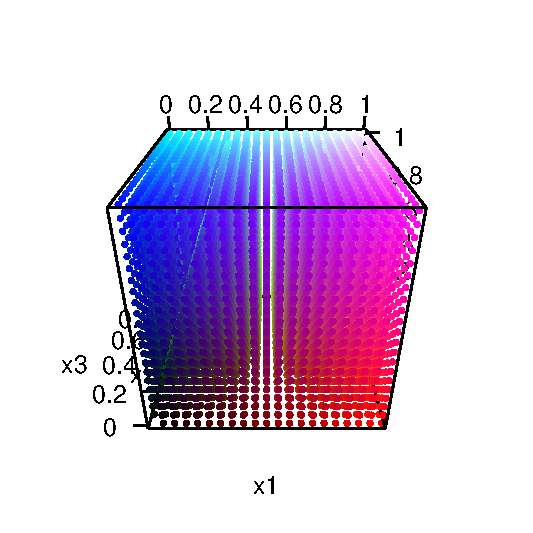
\includegraphics[width=.4\textwidth]{def3Dedge.pdf}
 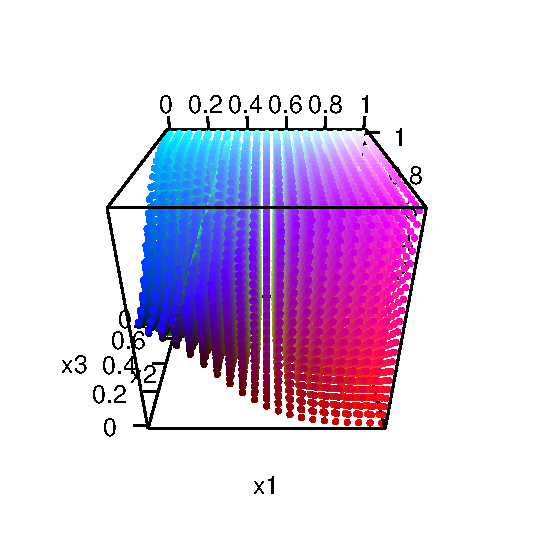
\includegraphics[width=.4\textwidth]{defAND.pdf}
 \caption{Warping for $c_1=R$ AND $c_2=1$. Left: original space (with the critical edge highlighted), right: distorted space. %Note that the axis has been rotated to show the shape of the distorted space.
 }\label{fig:def3Dedge}
\end{figure}

\paragraph{Affine conditions}
The ``AND'' condition can be generalized to the following affine formulation: 
$y$ is invariant w.r.t. $\x_J$ if $\mathbf{A} \x_I = \mathbf{b}$, 
with $\mathbf{A}$ a matrix of size $p \times \card(I)$ and $\mathbf{b}$ a vector of size $p$.
For the ``AND'' condition, we have $\mathbf{A} = \mathbb{I}_p$ and $\mathbf{b}=\cc_I$.
The warping function is the same as in Equation \ref{eq:and}, with now:
\begin{eqnarray}
  \alpha(\x_I,  \cc_I) &=& 1 - r_A(\mathbf{A} \x_I, \mathbf{b}).\label{eq:aff}
\end{eqnarray}
Note that choosing the range of the correlation $r_A$ is non-trivial. A possible solution is $\theta_A = \mathbf{A}^T \boldsymbol{\theta}_I$.

Figure \ref{fig:def3Daff} show the deformation of a cubic space with the condition: $y$ invariant w.r.t. $x_3$ if $x_1 = x_2$. 
 \begin{figure}[!ht]
 \centering
 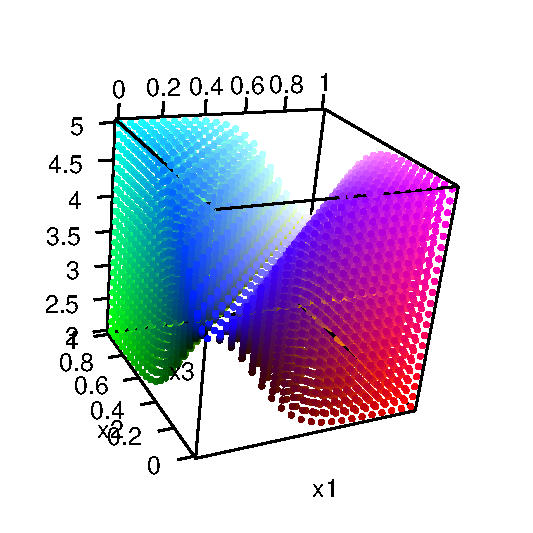
\includegraphics[width=.4\textwidth]{def3Daff.pdf}
 \caption{Warping for the affine condition: $y$ invariant w.r.t. $x_3$ if $x_1 = x_2$.}\label{fig:def3Daff}
\end{figure}

\section{Combining warpings}
\subsection{Independent conditions}
Now, we consider that we have a series of invariance conditions, defined with respect to sets $I_1, \ldots, I_n$ and corresponding $J_1, \ldots, J_n$.
% We assume that the invariance conditions are written only once for each variable, hence $J_k\cap J_l=\emptyset$, $1 \leq j\neq k \leq n$.
If $J_k\cap J_l=\emptyset$, $1 \leq j\neq k \leq n$ and $I_i\cap J_k = \emptyset$,  $1 \leq j,k \leq n$,
the set of warped variables are distinct from the set on which the conditions are written, 
the invariance conditions are written only once for each variable. In that case, 
the warpings can be applied independently.

\subsection{Combinations of simple conditions: ``OR'' invariance}
Now, we consider the case when $y$ is invariant w.r.t. a set $\x_J$ for different conditions on sets $I_1, \ldots, I_n$
(that, for $\x_{I_1}=\cc_{I_1}$ OR $\x_{I_2}=\cc_{I_2}$ OR $\ldots$).
If $J\cap I_i=\emptyset$, $1 \leq i \leq n$, the warping function we propose is:

\begin{equation}
 \forall j \in J, \quad \widetilde{x_j} = \overline{x_j} + \left( x_j - \overline{x_j}\right) \prod_{I \in \{I_1, \ldots, I_n \}}{\alpha_I}(\x_I, \cc_I)\label{eq:or0}. %\label{eq:orand}.
\end{equation}
% 
% \begin{eqnarray}
%  \forall j \in J, &\widetilde{x_j} =& \overline{x_j} + \left( x_j - \overline{x_j}\right) \prod_{i \in I} \alpha(x_i, c_{i})\label{eq:or0}.
% \end{eqnarray}
We see directly that the product of $\alpha$'s ensure that $\widetilde{x_j} = \overline{x_j}$
if any $x_i = c_i$, and the distortion reduces only when \emph{all} the $x_i$'s are far from the $c_i$'s.
% (instead of \emph{any} $x_i$, as in Equation \ref{eq:and}).
% In Equation \ref{eq:or2}, it is important to notice that the $x_k$'s are centered around the $c_k$'s instead of their mean, 
% to ensure that $\psi(\x_I, \x_J) = (\cc_I, \overline{\x_J})$ if any $x_i = c_i$.
Figure \ref{fig:def3DORs} shows a deformation of a cubic space when $x_3$ is not influent when $x_1$ or $x_2$ are minimal, when a Gaussian warping (exponential with $d=2$) is applied.
 \begin{figure}[!ht]
 \centering
 \includegraphics[width=.4\textwidth]{def3DORs.pdf}
 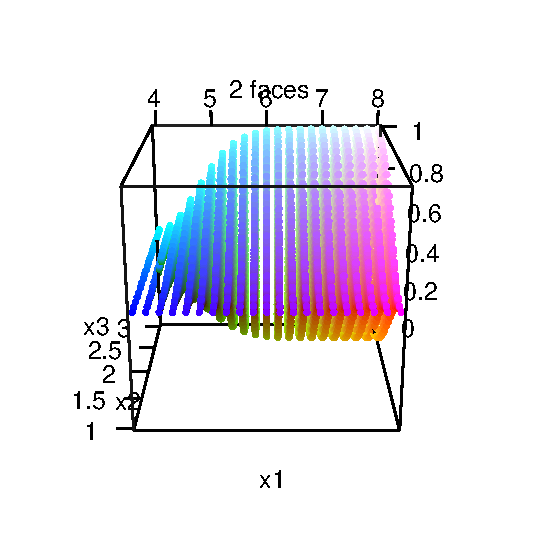
\includegraphics[width=.4\textwidth]{def3DOR2s.pdf}
 \caption{Warping for $c_1=4$ (left face of the cube) OR $c_2=1$ (front face). Left: original space, right: distorted space. %Note that the axis has been rotated to show the shape of the distorted space.
 }\label{fig:def3DORs}
\end{figure}

\paragraph{Multiple conditions on the same variable}
If $y$ is invariant w.r.t. $\x_J$ for any of the conditions $x_i = \{c_{i1}, \ldots, c_{in} \}$, the warping function is:
\begin{equation}
 \forall j \in J, \quad \widetilde{x_j} = \overline{x_j} + \left( x_j - \overline{x_j}\right) \prod_{k=1}^n \alpha(x_i, c_{ik}).\label{eq:mult}
\end{equation}
An example if given in Figure \ref{fig:def2Dxx}, using a Gaussian attenuation.
% Note that this approach is closely related to considering toric topologies; 
% but it differs in the sense that . 

Note that the $c_{ik}$'s can take any value and not necessarily a boundary: %Figure \ref{fig:def2Dother} 
here we used $c_{11}=4$ (lower bound) and $c_{12}=7$ (in the middle of the domain of $x_1$).
On can notice that far away from the critical conditions, the mesh is undeformed locally AND globally, 
and in particular the distance between the far left and far right of the figure is unchanged by the warping.

\begin{figure}[!ht]
 \centering
 \includegraphics[width=.8\textwidth]{def2Dxx.pdf}
 \caption{Warping for two critical values for $x_1$.}\label{fig:def2Dxx}
\end{figure}

% \paragraph{``OR+AND'' invariances}
% More complex logical structures can be taken into account, for instance: $y$ is invariant w.r.t. $\x_J$ if 
% at least one $\x_i = \cc_i$, $i \in I_1$ and at least one $\x_k = \cc_k$, $k \in I_2$.
% In that case, we first rewrite the condition as an ``OR'' one: ($\x_i = \cc_i$ AND $\x_k = \cc_k$) OR ($\ldots$ AND $\ldots$) OR $\ldots$, then
% we simply combine Equations \ref{eq:or0} and \ref{eq:and} into:
% \begin{equation}
%  \forall j \in J, \quad \widetilde{x_j} = \overline{x_j} + \left( x_j - \overline{x_j}\right) \prod_{I \in \{I_1, \ldots, I_n \}}{\alpha_I}(\x_I, \cc_I)\label{eq:orand}.
% \end{equation}

\subsection{``Circular'' conditions}
Difficulty only arises when some variables appear in both $I_l$'s and $J_m$'s sets. Take for instance a ``reciprocal'' condition, 
e.g., $y$ is invariant w.r.t. $\x_J$ when $\x_I=\cc_I$, and invariant w.r.t. $\x_I$ when $\x_J=\cc_J$.
In that case, applying independently warping functions would lead to: 
\begin{eqnarray*}
 \psi(\cc_I, \x_J, \x_{-IJ}) &=& (\cc_I, \overline{\x_J}, \x_{-IJ}),\\
 \psi(\x_I, \cc_J, \x_{-IJ}) &=& (\overline{\x_I}, \cc_J, \x_{-IJ}),\\
 \text{but: } \psi(\cc_I, \cc_J, \x_{-IJ}) &=& (\cc_I, \cc_J, \x_{-IJ}),
\end{eqnarray*}
which induces a discontinuity.

In that case, a simple solution is to fix the non influent variable to its critical value instead of its average, hence applying:
\begin{eqnarray}
%  \forall j \in J, &\widetilde{x_j} =& \overline{x_j} + \left( x_j - \overline{x_j}\right) \prod_{i \in I} \alpha(x_i, c_{i})\label{eq:or1},\\
 \forall k \in K= \left( \cup_{1 \leq l \leq n} I_l \right) \cap \left(\cup_{1 \leq m \leq n} J_m \right), &\widetilde{x_k} =& c_k + \left( x_k - c_k\right) \prod_{i \in I_k} \alpha(x_i, c_{i})\label{eq:or2}.
\end{eqnarray}

\paragraph{Remark} This formula does not apply when $x_k$ takes multiple critical values (Equation \ref{eq:mult}) or in the affine case (Equation \ref{eq:aff}).
% Unfortunately, there does not seem to be an easy solution for those cases.

We first show the deformations on a 2D space on Figure \ref{fig:def2DOR}, where the two critical values are on the boundaries of $x_1$ and $x_2$, and on Figure \ref{fig:def2DT},
where one critical value is in the middle of the $x_1$ space. Here, the warping of Equation \ref{eq:or2} is applied on each variable ($K=\{1,2\}$). 
Again, except for the linear warping, the local topology is preserved far from the critical edges. 
On Figure \ref{fig:def2DT}, we also see that long-range distances are also unchanged.
A GP realization is given on Figure \ref{fig:simu2DT}. The ``T-shaped'' invariance is ensured, and the GP is stationary far from the critical values.

\begin{figure}[!ht]
\centering
 \includegraphics[width=.8\textwidth]{def2DOR.pdf}
 \caption{Three deformations of a 2D space, with invariance at $x_1=8$ OR $x_2=1$, highlighted with larger lines.}\label{fig:def2DOR}
\end{figure}

\begin{figure}[!ht]
 \centering
 \includegraphics[width=.8\textwidth]{def2DT.pdf}
 \caption{Warping for a T-shaped ``OR'' invariance.}\label{fig:def2DT}
\end{figure}

\begin{figure}[!ht]
 \centering
 \includegraphics[trim=2mm 45mm 2mm 45mm,clip,width=.4\textwidth]{simu2DT.pdf}
 \caption{GP realization for a T-shaped ``OR'' invariance.}\label{fig:simu2DT}
\end{figure}

Then, we consider a cubic space with the following circular conditions:
\begin{itemize}
 \item $y$ is invariant w.r.t. $x_2$ if $x_1=4$;
 \item $y$ is invariant w.r.t. $x_3$ if $x_2=1$;
 \item $y$ is invariant w.r.t. $x_1$ if $x_3=0$.
\end{itemize}
All critical values correspond to the lower bounds of the variables.
Equation \ref{eq:or2} is applied to each variable, hence with $K=\{1,2,3\}$, $C=[4,1,0]$ and $I_1=3$, $I_2=1$, and $I_3=2$. 
The original and distorted space is shown in Figure \ref{fig:def3Dcirc}.

 \begin{figure}[!ht]
 \centering
 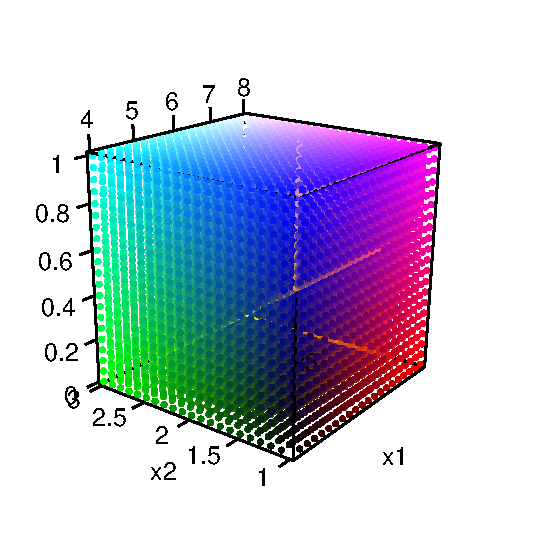
\includegraphics[width=.4\textwidth]{def3Dcirc1.pdf}
 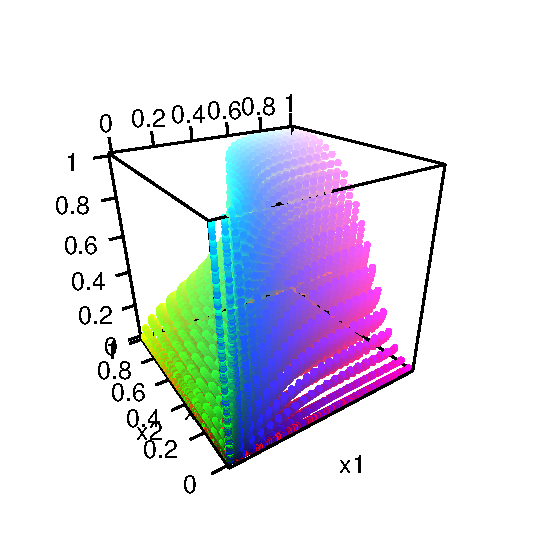
\includegraphics[width=.4\textwidth]{def3Dcirc2.pdf}
 \caption{Warping with circular conditions. Left: original space, right: distorted space.}\label{fig:def3Dcirc}
\end{figure}

\subsection{``Circular'' affine conditions}
In this section, we report experimental solutions that appear to work on 3D cases.
We consider a series of three test cases, on the design space $x_1 \in [1,4]$, $x_2 \in [2,3]$ and $x_1 \in [0,2]$,
defined by the following conditions:
\begin{itemize}
 \item (affine + simple circular conditions) $y$ is invariant w.r.t. $x_1$ if $2 x_2=3 x_3$, and  w.r.t.  $x_3$ if $x_1=1$;
 \item (2 affine circular conditions) $y$ is invariant w.r.t. $x_1$ if $2 x_2=3 x_3$, and  w.r.t.  $x_2$ if $x_1=2 x_3$;
 \item (3 affine circular conditinos) $y$ is invariant w.r.t. $x_1$ if $2 x_2=3 x_3$, w.r.t.  $x_3$ if $x_1=1$ and w.r.t. $x_3$ if $3 x_1=4 x_2$.
\end{itemize}
Note that the design space is voluntarily different from the unit cube.

In the first case, we applied:
\begin{eqnarray*}
 \widetilde{x_1} &=& c_1 + \left( x_1 - c_1\right) \alpha(x_1, c_1) \alpha(2 x_2 - 3 x_3, 0) \\
 \widetilde{x_3} &=& c_3 + \left( x_3 - c_3\right) \alpha(x_i, c_1) \alpha(2 x_2 - 3 x_3, 0).
\end{eqnarray*}

In the second case, we applied:
\begin{eqnarray*}
 \widetilde{x_1} &=& c_1 + \left( x_1 - c_1\right) \alpha(x_1, c_1) \alpha(2 x_2 - 3 x_3, 0) \\
 \widetilde{x_2} &=& c_2 + \left( x_1 - c_2\right) \alpha(x_1, c_1) \alpha(2 x_2 - 3 x_3, 0) \\
 \widetilde{x_3} &=& c_3 + \left( x_3 - c_3\right) \alpha(x_i, c_1) \alpha(2 x_2 - 3 x_3, 0).
\end{eqnarray*}

In the third case, we applied:
\begin{eqnarray*}
 \widetilde{x_1} &=& c_1 + \left( x_1 - c_1\right) \alpha(x_1, c_1) \alpha(2 x_2 - 3 x_3, 0) \alpha(3 x_1 - 4 x_2, 0) \\
 \widetilde{x_2} &=& c_2 + \left( x_1 - c_2\right) \alpha(x_1, c_1) \alpha(2 x_2 - 3 x_3, 0) \alpha(3 x_1 - 4 x_2, 0) \\
 \widetilde{x_3} &=& c_3 + \left( x_3 - c_3\right) \alpha(x_i, c_1) \alpha(2 x_2 - 3 x_3, 0) \alpha(3 x_1 - 4 x_2, 0).
\end{eqnarray*}

On all cases, $C$ was chosen within the intersection of the critical plans: for instance in the second example,
at the intersection of $2 x_2=3 x_3$, and  $x_1=2 x_3$. Since this intersection is a segment, we took $C$ as the 
the average of the intersection.

Figure \ref{fig:3cases}

\begin{figure}[!ht]
 \centering
 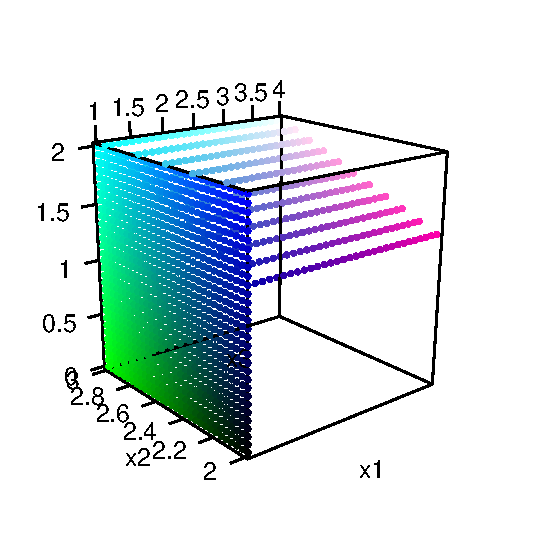
\includegraphics[width=.4\textwidth]{plan2.pdf}
 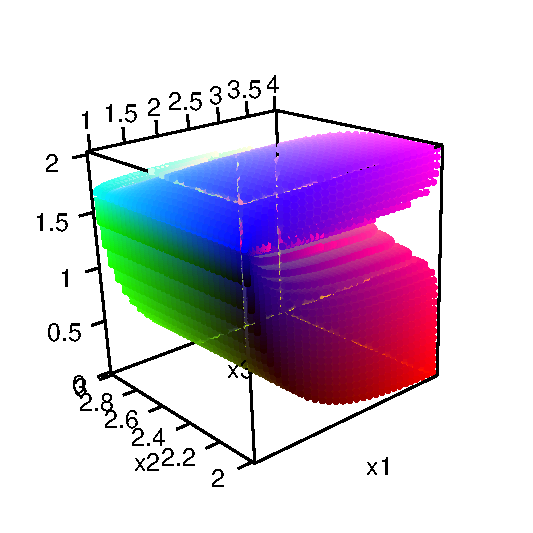
\includegraphics[width=.4\textwidth]{warp2.pdf}
  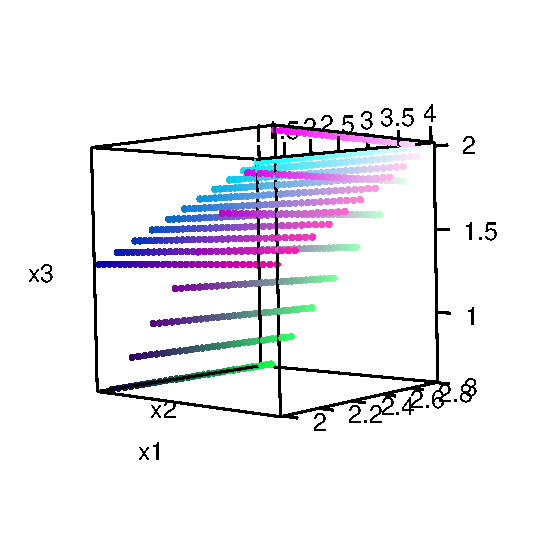
\includegraphics[width=.4\textwidth]{plan3.pdf}
 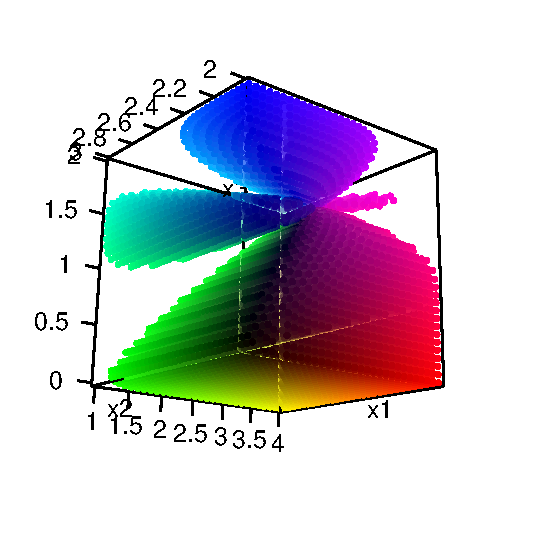
\includegraphics[width=.4\textwidth]{warp3.pdf}
  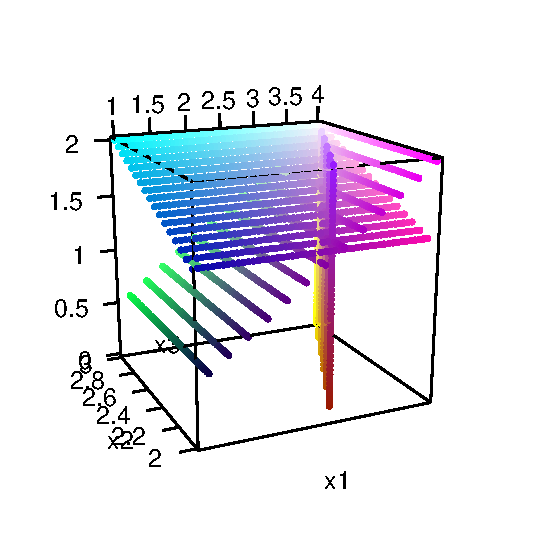
\includegraphics[width=.4\textwidth]{plan4.pdf}
 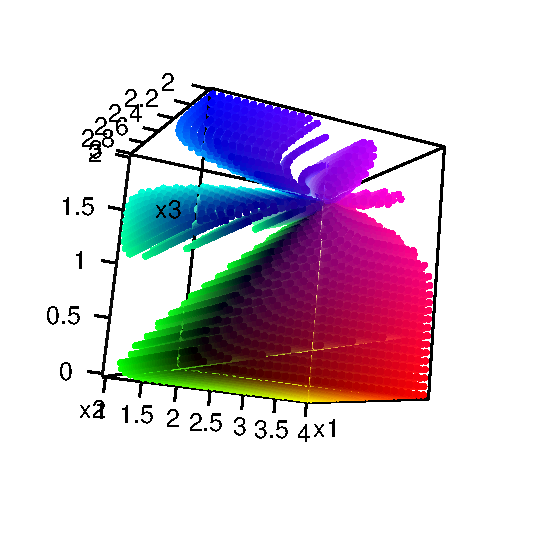
\includegraphics[width=.4\textwidth]{warp4.pdf}
 \caption{Warpings for three different cases with circular conditions. Left: critical plans, right: corresponding distorted space.}\label{fig:3cases}
\end{figure}

\subsection{A complex example}
Finally, we show the deformations on a cubic space, with the following conditions:
\begin{itemize}
 \item $y$ is invariant w.r.t. $x_3$ if $x_1=4$ or $x_2=1$
 \item $y$ is invariant w.r.t. $x_2$ if $x_1=4$ 
 \item $y$ is invariant w.r.t. $x_1$ if $x_2=1$ 
\end{itemize}
Equation \ref{eq:or0} is applied to $x_3$ ($j=3$, $I=\{1,2\}$), while Equation \ref{eq:or2} is applied to $x_1$ and $x_2$ ($K=\{1,2\}$,
$I_1=2$ and $I_2=1$), with a Gaussian warping.
Invariance occurs on the left and front faces of the cube ($x_1$ and $x_2$ to their minimum, Figure \ref{fig:def3D2faces}, left).
In the resulting topology, those two faces collapse into a single point as desired. 
Note however the large difference with the ``AND'' condition in Figure \ref{fig:def3Dedge}, for which the 
cubic topology is mostly preserved except close to the critical edge.

 \begin{figure}[!ht]
 \centering
 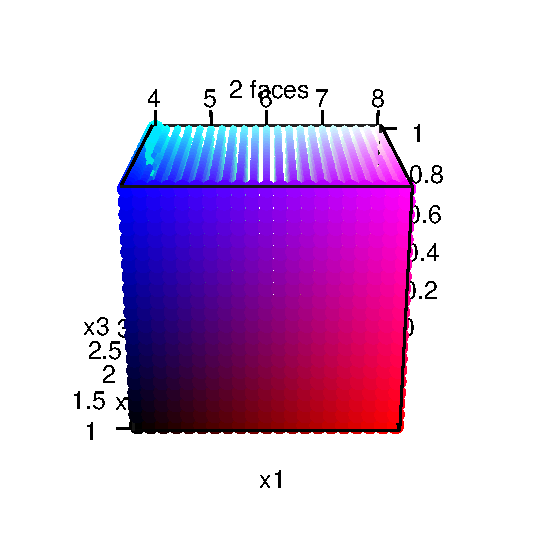
\includegraphics[width=.4\textwidth]{def3DOR.pdf}
 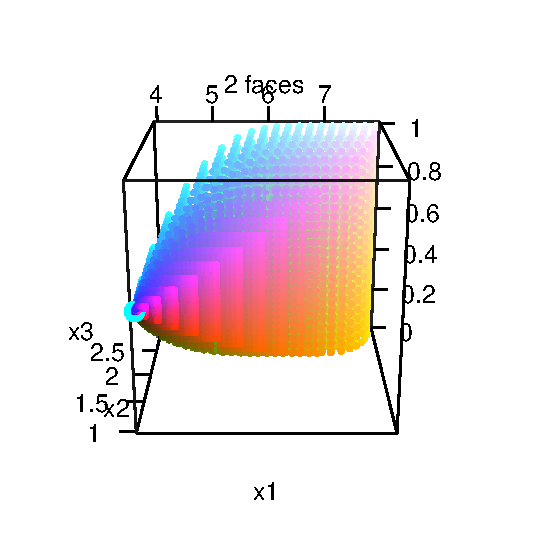
\includegraphics[width=.4\textwidth]{def3DOR2.pdf}
 \caption{Warping for $x_2$ and $x_3$ inactive if $c_1=4$ and $x_1$ and $x_3$ inactive if $c_2=1$. Left: original space, right: distorted space. }\label{fig:def3D2faces}
\end{figure}

\end{document}
